
\graphicspath{{images/}}

\subsection{Spark use-case}


\subsection{OpenStack use-case}
\label{subsec:openstack}

OpenStack~\cite{os:7923796} is the de-facto open-source solution to address the
IaaS level of the Cloud paradigm. Since $2010$, its community has gathered
nearly $700$ organizations (such as Google, IBM or Intel) and has produced more
than $20$ million lines of code. Its adoption is still growing in various
domains such as public administrations, e-commerce and science\footnote{See
\url{http://superuser.openstack.org/} for further information.}.

OpenStack is a large distributed software that brings together almost $100$
% TODO: Each of which en début de phrase ?
software projects. Each of which is in charge of a specific aspect of the
infrastructure management (\eg provision virtual machines, provide them with
storage, interconnect them through networks) and their cooperation is the key to
provide the features required by Cloud management.
%
Those projects are themselves composed of several software modules that are
responsible for very specific tasks (\eg placement, hypervisors, regarding
virtual machine management). While they are not all mandatory to deploy an
operable IaaS, $250$ software modules are available in those projects.
%
An OpenStack instance is a composition by the operator of those modules, which
cooperate to respond to her requirements. For instance, the operator may need
services to manage virtual rather than bare-metal machines, object storage
rather than file-systems, while VLAN networks and billing services may not be
desired in her use-case. As defined in the large OpenStack documentation, each
software module has its own commissioning process, and may depend on other
module commissioning.
%
The deployment of a typical OpenStack instance implies thus many software
modules whose commissioning process is characterized by a large amount of tasks
and interplays. As a consequence, the commissioning process of OpenStack is
complex to understand and can be very long when tasks are executed sequentially.
%
In the following, we show how the commissioning process of each OpenStack
project can be transcribed as a \mad component. Leveraging \mad enables us to
abstract tasks as transitions and express task and component coordination. As a
consequence, the \mad representation improves the global commissioning process
understandability, and can be used to reduce commissioning time by exploiting
node, intra and inter-component parallelism.
% express module interplays can help new developers to better understand both
%   code and workfow
% madeus can be used to express parallel tasks and understand module interplay

\subsubsection{Presentation}

\begin{table*}
  \begin{center}
    
\begin{tabular}{|c|c|c|c|c|}
   \hline
   & Roles & Places & Transitions & Ports \\
   \hline
   Nova & Manages compute instances (\eg Virtual machines) & 5 & 8 & 8\\
   Glance & Compute image store & 3 & 4 & 7\\
   Neutron & In charge of network resources & 3 & 4 & 7\\
   MariaDB & An SQL server used by most projects to store persistent
    information & 4 & 5 & 4\\
   Keystone & Manage user authentication, authorization and service
    discovery & 3 & 2 & 4\\
   RabbitMQ & The message bus for inter-service communication & 2 & 1 & 3\\
   HAProxy & Load-balances the requests to OpenStack controllers & 2 & 1 & 7\\
   OpenVSwitch & Virtualizes network functions & 3 & 1 & 2\\
   MemCached & Caches ephemeral data for most OpenStack projects & 2 & 1 & 2\\
   Facts & Collects informations about every nodes & 2 & 1 & 1\\
   Common & Common utilities (\eg cron, fluentd: a metric collector for logging)
    & 3 & 2 & 2\\
%   \hline
%   Total & 32 & 30 & 47 & \\
%   \hline
%   & Places & Transitions & Ports & Roles\\
%   \hline
%   Nova & 5 & 8 & 8 & Manage compute instances (\eg Virtual machines)\\
%   Glance & 3 & 4 & 7 & Compute image store\\
%   Neutron & 3 & 4 & 7 & In charge of network resources\\
%   Keystone & 3 & 2 & 4 & Manage user authentication, authorization and service
%    discovery\\
%   MariaDB & 4 & 5 & 4 & An SQL server used by most projects to store persistant
%    information\\
%   RabbitMQ & 2 & 1 & 3 & The message bus for inter-service communication\\
%   HAProxy & 2 & 1 & 7 & Load-balances the requests to OpenStack API services\\
%   OpenVSwitch & 3 & 1 & 2 & Virtualizes network functions\\
%   MemCached & 2 & 1 & 2 & Caches ephemeral data for most OpenStack projects\\
%   Facts & 2 & 1 & 1 & Collects inforamtions about every nodes\\
%   Common & 3 & 2 & 2 & Common utilities (\eg cron, fluentd: a
%   metric collector for logging) \\
   \hline
   Total & & 32 & 30 & 47\\
   \hline
\end{tabular}


    \caption{Number of places, transitions, ports and roles for each \mad component
        of the OpenStack assembly of Figure~\ref{fig:full}.}
    \label{tab:os}
  \end{center}
\end{table*}

\kolla is one of the most popular project for deploying OpenStack in production.
It relies on \ansible to deploy OpenStack's modules as \docker containers, and
will be considered as our reference in the rest of this section. It is highly
opinionated out-of-the-box, allowing operators to quickly deploy a basic
OpenStack instance, but enables complete customization for advanced
administrators. As a consequence, the use-case described in this section
corresponds to the default \kolla deployment, which provides the essential
mechanisms to operate an infrastructure with OpenStack.
%
To compare the performance of \kolla and \mad, we have defined $11$ \mad
components based on the \ansible roles defined in \kolla's playbooks. Their
names are built for most of them on the OpenStack project they deploy.
\Cref{tab:os} lists these components and indicates which aspect of the Cloud
management they are in charge of. Furthermore, some \mad metrics are diplayed
(\ie the number of places, transitions and ports).
%
In this table, when the number of transitions is greater or equal to the number
of places, it means that \mad can be leveraged to express parallel transitions.
Also, the more ports, the more \mad is able to coordinate interplays during the
deployment. As depicted in \cref{tab:os}, Nova, Glance, Neutron and MariaDB are
components of particular interests since they contain more transitions and ports
than the others.

\begin{figure}
  \begin{center}
    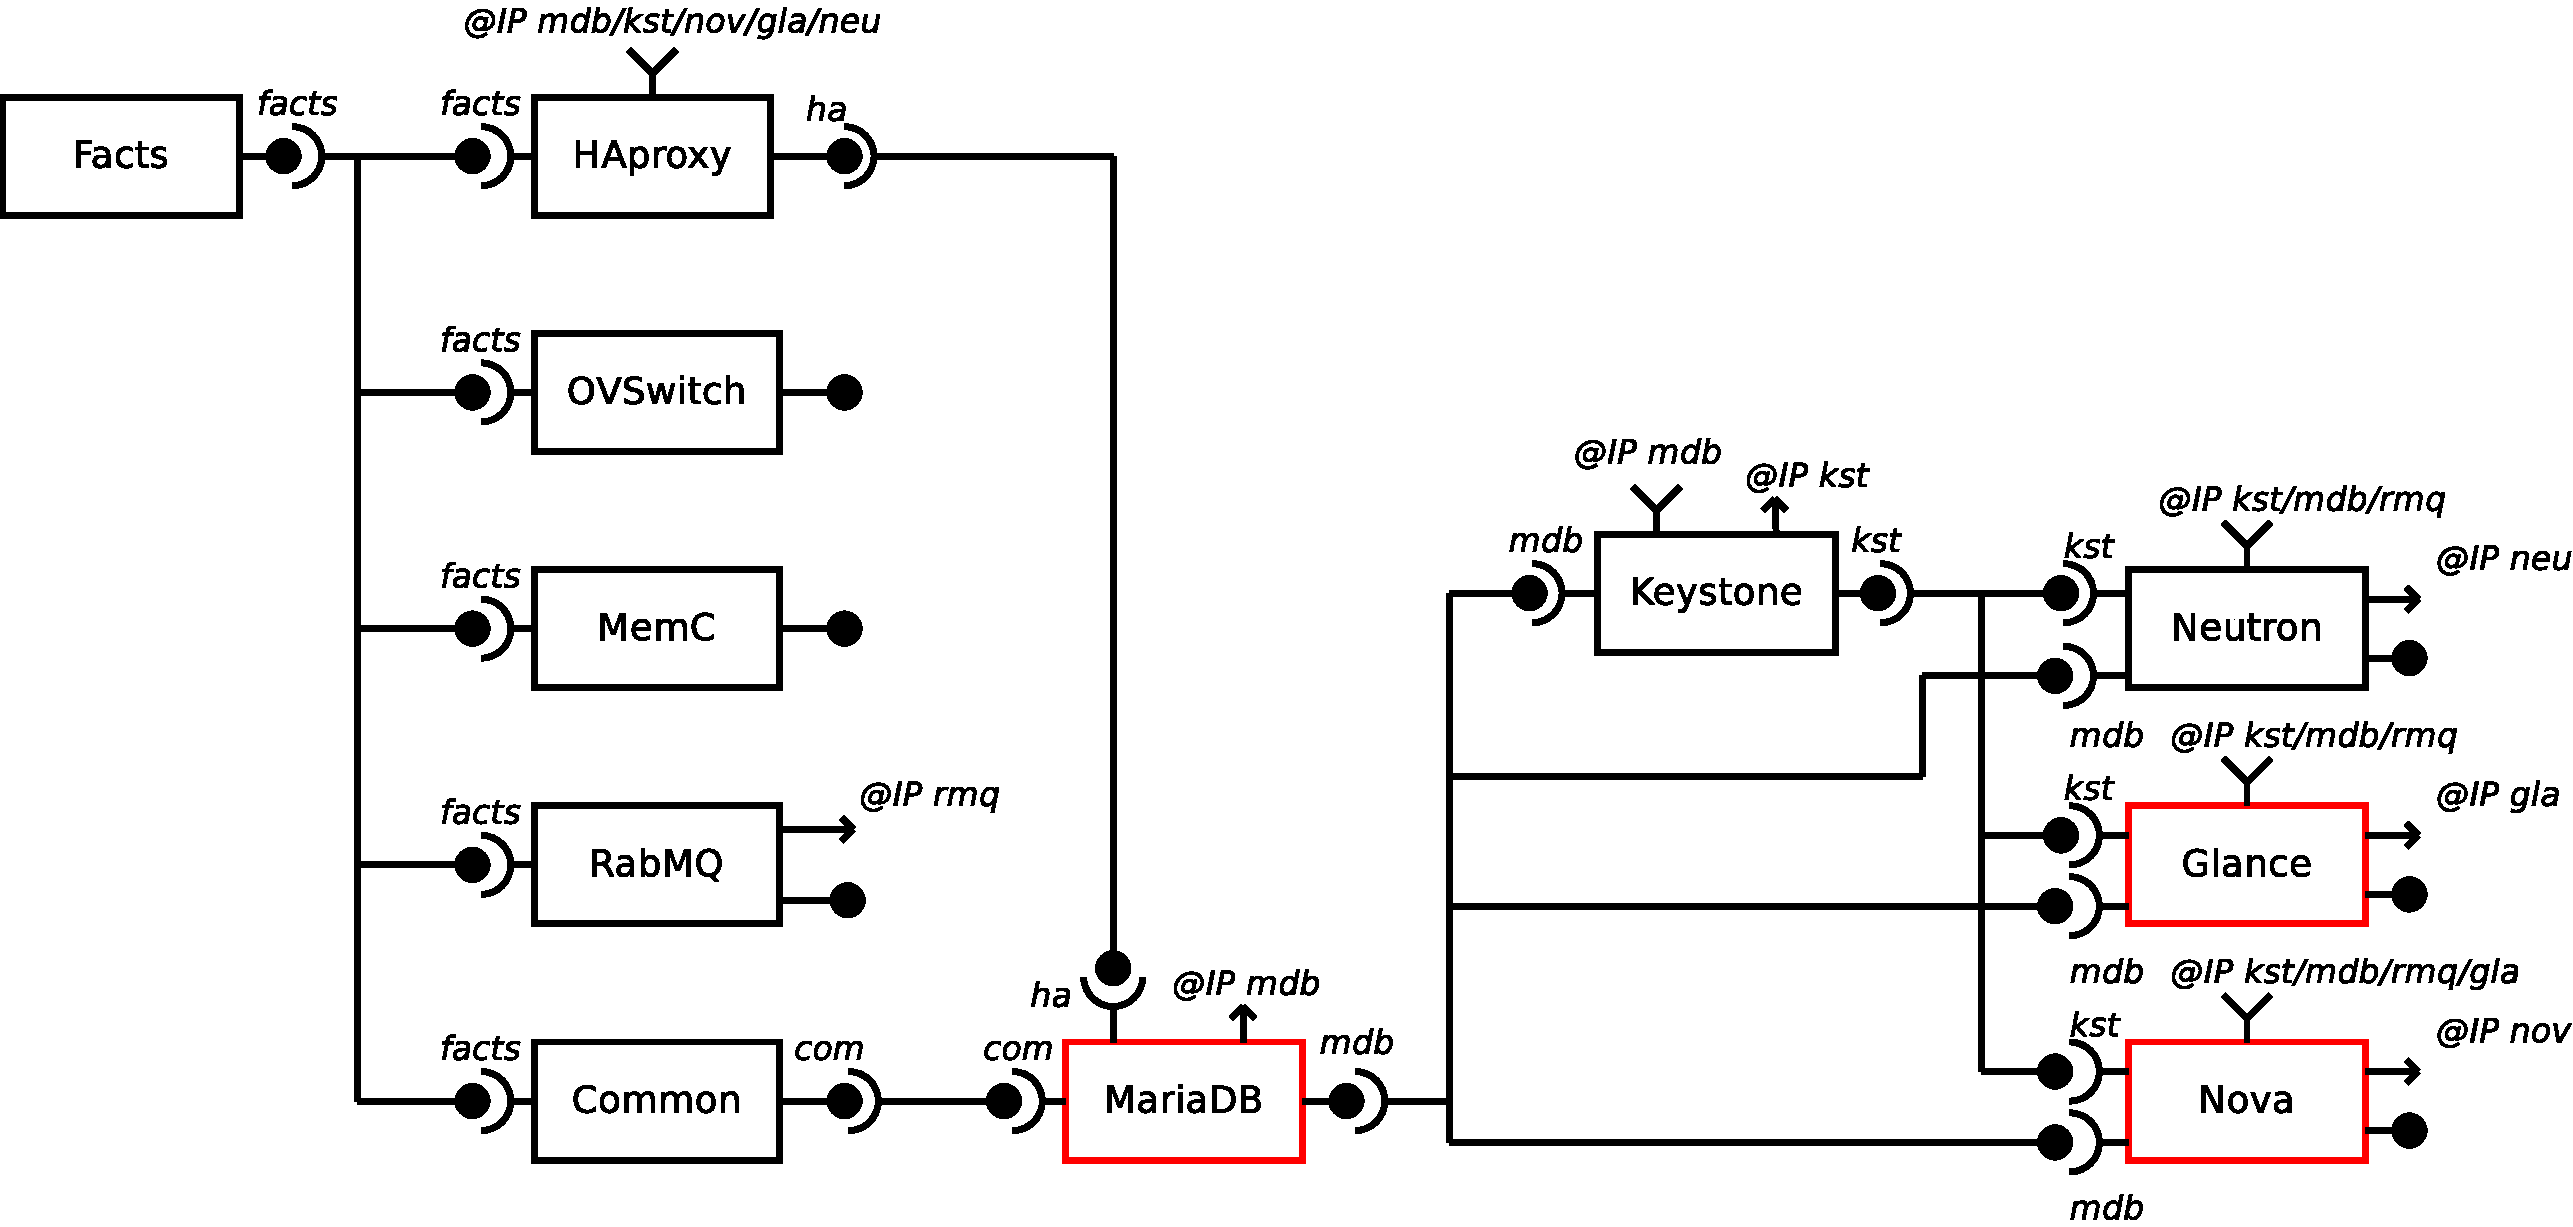
\includegraphics[width=0.5\textwidth]{./images/full.pdf}
    \caption{Simplified \mad assembly of the \kolla-based OpenStack deployment
    containing $11$ components. Connections between data ports are not depicted.
    Red components are detailed in \cref{fig:sub}.}
    \label{fig:full}
  \end{center}
\end{figure}
% TODO: Refaire cette figure en SVG pour la faire tenir sur une colonne avec
% police du papier pour que ce soit lisible

\Cref{fig:full} depicts the use-case from the operator viewpoint (\ie at the
level of the \mad assembly). For the sake of simplicity and readability, the
connections between data ports are not represented. This figure helps to
understand the high-level interplays between components. For instance, Neutron,
Glance and Nova require Keystone, while Keystone requires itself a database (\ie
MariaDB) for its commissioning process.
%MariaDB relies itself on HAProxy for being reachable through a virtual IP address.
Regarding the separation of concerns, the operator does not need to understand
component internals. She just needs to compose the desired component by listing
them and connecting them. As a consequence, a component can be replaced by
another one if they expose the same interface. For instance the operator could
replace MariaDB with MySQL: another component which also implements a database
by exposing the same ports.
% at least the same ports that are used by MariaDB

\begin{figure*}[t]
  \begin{center}
    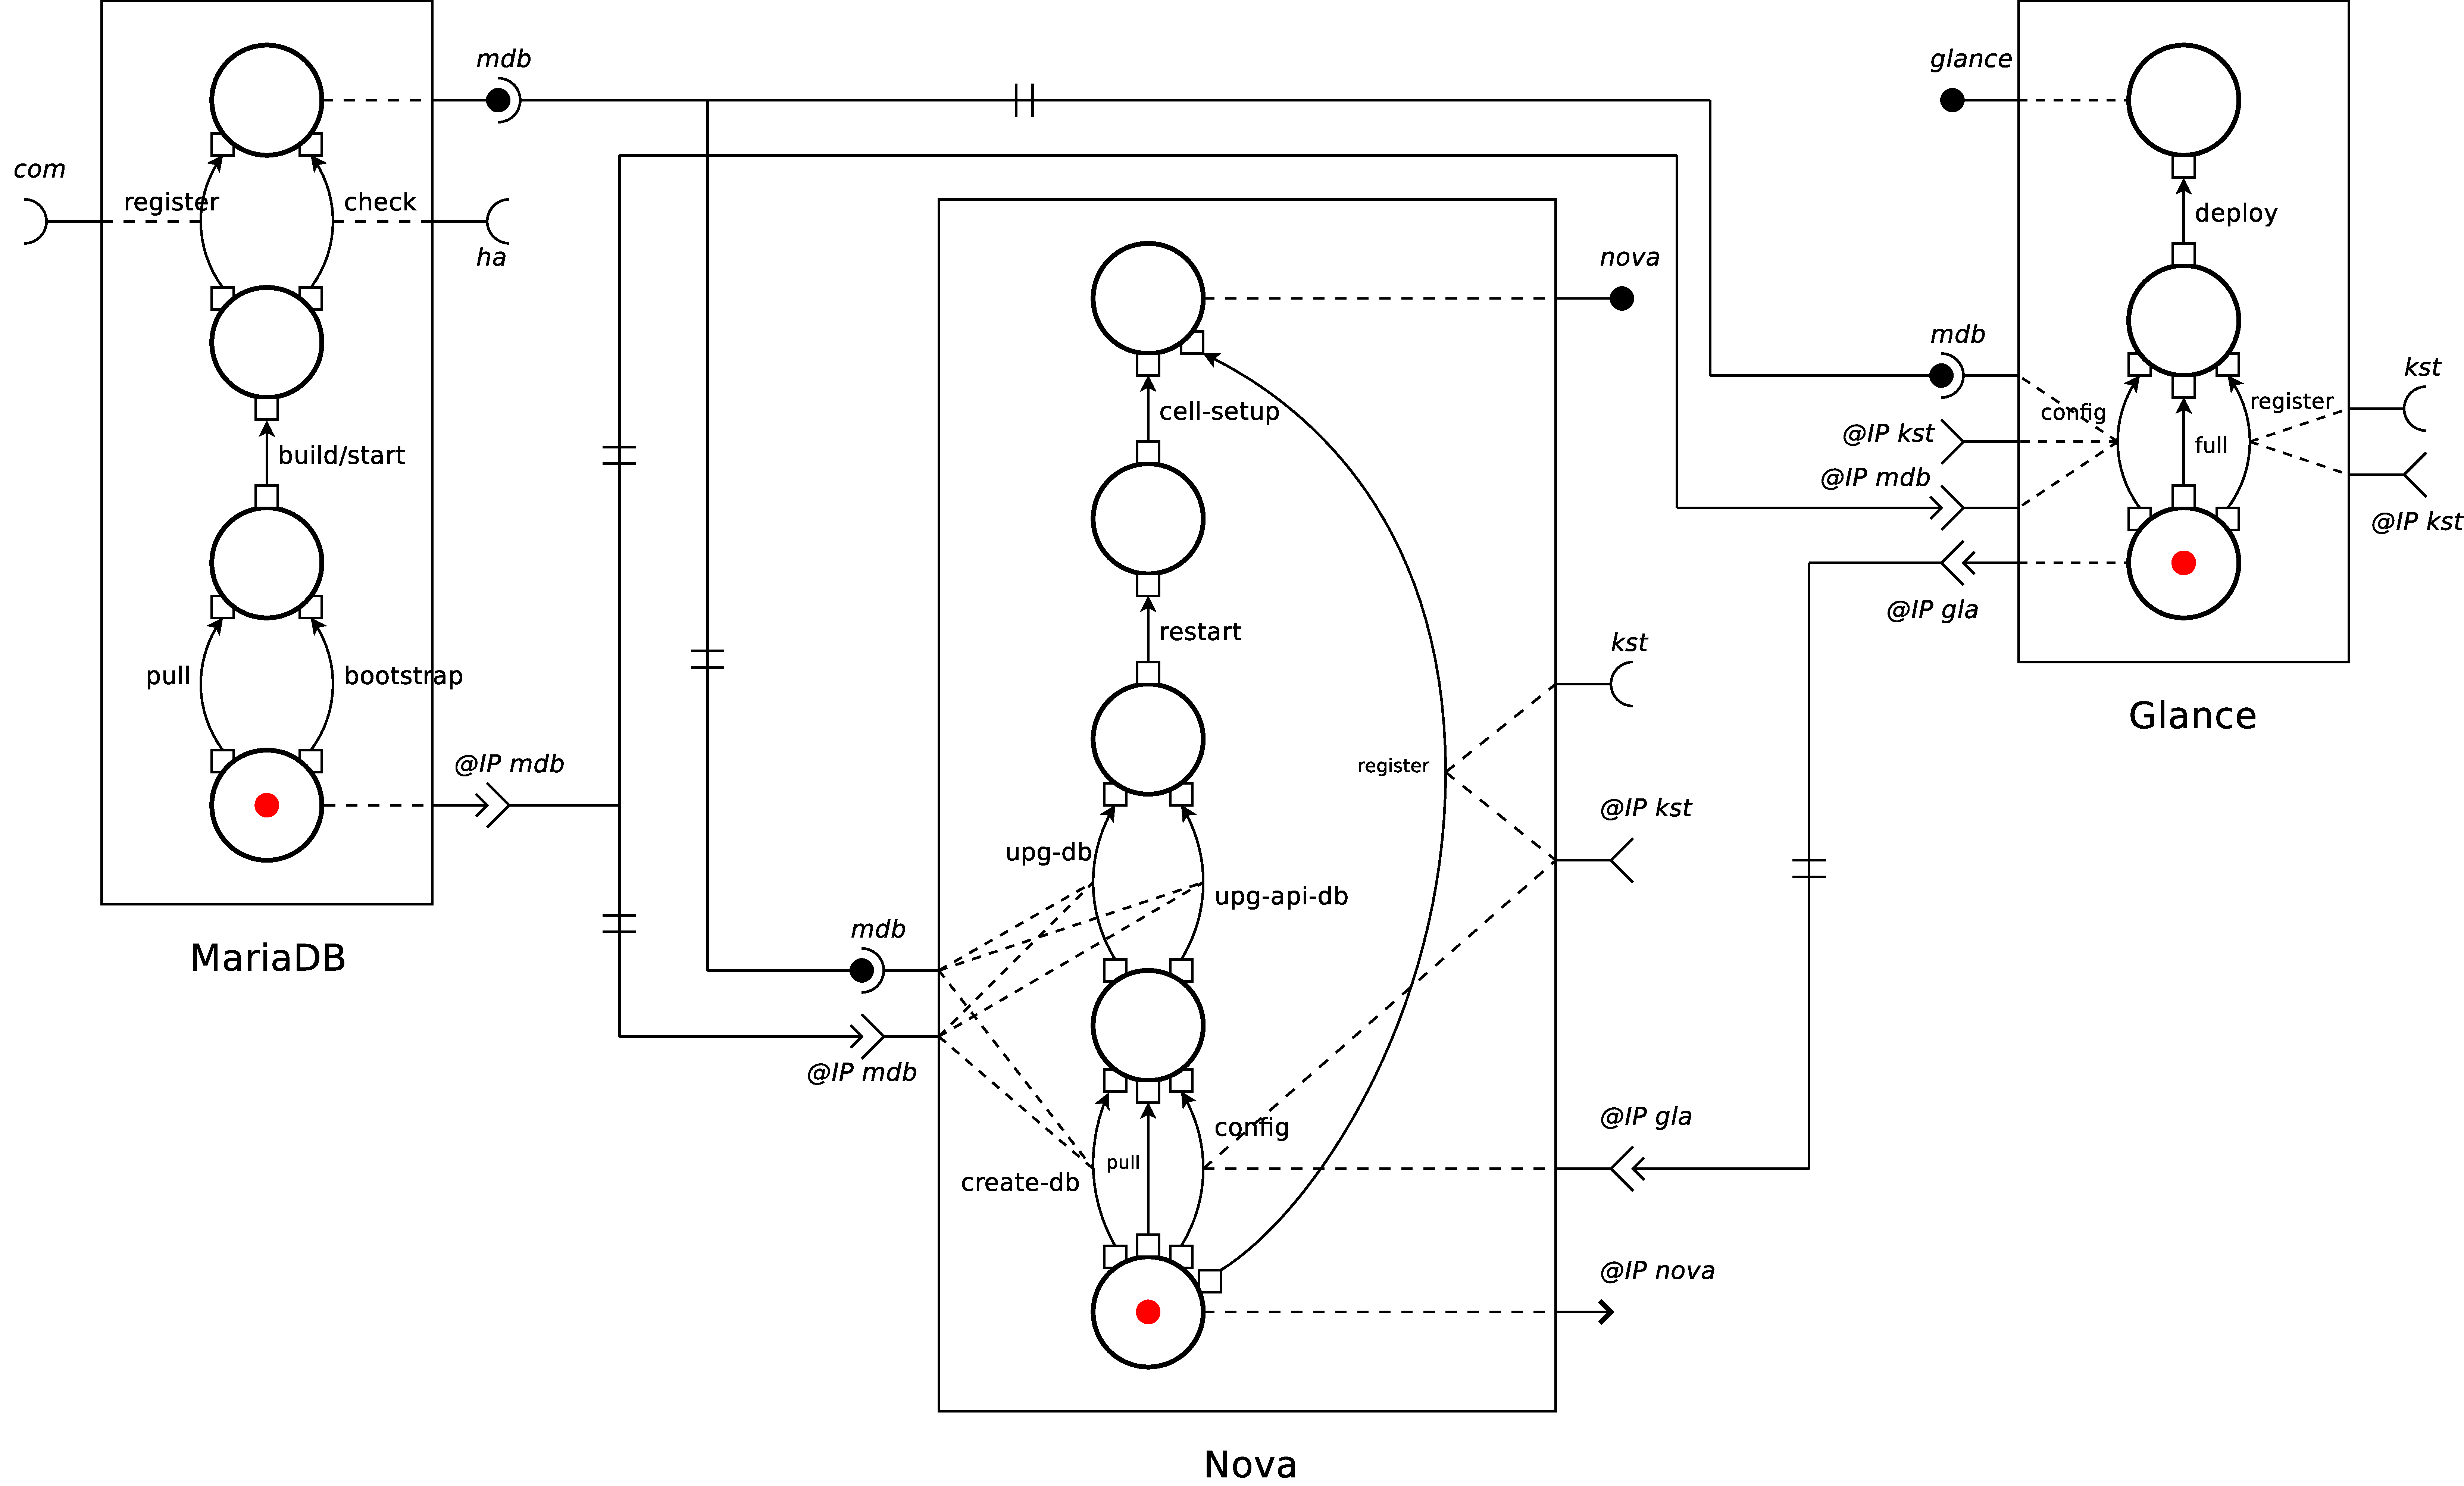
\includegraphics[width=0.8\textwidth]{./images/sub.pdf}
    \caption{A detailed sub-part of the previous component assembly to deploy
    OpenStack. The three colored components of \cref{fig:full} are detailed by
    using \mad. Black, green, blue and red tokens represent different scenarios
    during the deployment process.}
    \label{fig:sub}
  \end{center}
\end{figure*}
%TODO: Il manque les tokens de couleur dont la caption fait référence
%TODO: J'aurais peut être représenté Keystone à la place de MariaDB
%   1. Est-ce utile de dire que mariadb ici est différent de mariadb avant et
%   pas risqué pour embrouiller le message ?
%   2. Register est une transition liée à Keystone qui est très intéressante
%   quand on examine Nova (transition indépendante des autres)

We now study our use-case from the developer viewpoint, focusing on the three
colored components from \cref{fig:full}: MariaDB, Nova and Glance.
\Cref{fig:sub} depicts the internals and interplays of these components.
%
% First, the MariaDB component showed in this figure is different from the one
% depicted in \cref{fig:example}. The component here has additional content: (i)
% the transition \emph{register} that relies on the Common component; (ii) the
% transition \emph{check} that relies on HAProxy (in our use-case, MariaDB is
% reachable from HAProxy's virtual IP address). This illustrates that according to
% the type of deployment the developer or the operator aims at performing, the
% component internals may need to be modified.  Thus, it shows that being able to
% customize a component internals may be needed to improve both the expressiveness
% and efficiency of a deployment.
% TODO: récupérer de Middlware, je ne suis pas sûr que l'on garde en fonction du
% discours du papier
The dependencies previously observed at the assembly level are more
detailed at the developer level.
First, if we isolate Nova and Glance for instance, while \cref{fig:full} let us
think that Glance must be deployed before Nova, it is clear here that once Nova
obtains Glance's IP address (provided by the first place in Glance), both
components can be deployed in parallel. This shows how \mad can be leveraged for
inter-component parallelism.
%TODO: à voir si c'est pas redondant avec ce qui a été dit dans la présentation mad
Second, as we discussed before, it seemed in \cref{fig-full} that
MariaDB must be deployed before Keystone, and Keystone before
Neutron/Glance/Nova. However, with the \mad representation depicted in
\cref{fig:sub}, we understand that only the \emph{register} transition of Glance
and Nova requires the service catalog Keystone to be available (\ie to register
themselves in the catalog). We can see on the figure that other tasks can be
executed in parallel while \emph{register} waits for Keystone (\eg for Nova,
this transition is independent for all the other ones). Similarly,
\cref{fig:sub} depicts for each component many parallel transitions showing how
\mad can be leveraged for intra-component parallelism in this use-case.

\subsubsection{Experimental Setup and Parameters}
% Ici on décrit nos paramètres et le testbed
This section defines first the experimental setup: (i) how modules are
distributed among nodes and (ii) the testbed characteristics. Then we describe
the different parameters used during our experimentation: (iii) the assemblies
we designed to compare our contribution with the related work and (iv) the way
\docker images are fetched by nodes.

\paragraph{Node roles and module distribution}
Each of the $11$ components defined earlier in \kolla is in charge of a
OpenStack project. As we said previously, each OpenStack project contains
multiples software modules. Hence, each component actually deploys different
modules ($36$ in total). A basic multi-node \kolla deployment targets three
nodes. First, the \emph{Control} node which hosts control services, APIs and
databases, commissions $16$ services. The second one is the \emph{Network} node
that hosts network agents and HAProxy, and contains $11$ services. Finally, the
\emph{Compute} node, in charge of compute services and where guest VMs live,
hosts $9$ services.

\begin{table}
  \begin{center}
    \small
    
\begin{tabular}{|c|c|c|c|}
   \hline
   Cluster & CPU & Memory & Network\\
   \hline
   Nova & 2 x Intel Xeon E5-2620 v4 & 64GB & 10Gbps\\
   (lyon) & 8 cores/CPU &  & \\
   \hline
   Taurus & 2 x Intel Xeon E5-2630 & 32GB & 10Gbps\\
   (lyon) & 6 cores/CPU & & \\
   \hline
   Sol & 2 x AMD Opteron 2218 & 4GB & 1Gbps\\
   (sophia) & 2 cores/CPU & &\\
   \hline
\end{tabular}


    \caption{Grid'5000 cluster configurations.}
    \label{tab:g5k}
  \end{center}
\end{table}

\paragraph{Testbed and resource provisioning}
Our evaluations have been conducted on two clusters from the experimental
platform Grid'5000\footnote{\url{www.grid5000.fr}}: \ecotype and \nova. \Cref
shows the hardware configuration for both clusters. The cluster \ecotype has a
better hardware configuration than the latter, regarding CPU, memory and network
interfaces, as detailed in the table. To design reproducible benchmarks, we
used EnosLib\footnote{\url{https://gitlab.inria.fr/discovery/enoslib}}, a
library to build experimental frameworks on multiple testbeds (\eg Grid5000,
LibVirt), and
Execo\footnote{\url{http://execo.gforge.inria.fr/doc/latest-stable/index.html}},
another library for prototyping experiments. Since \kolla, our reference, does
not manage resource provisioning, we do not include this phase in the use-case,
nor in our benchmark. Even if resource provisioning could be managed by \mad,
this step is left to EnosLib.
% TODO à voir si ça n'a pas été présenté par Maverick avant

\paragraph{Assemblies}
Our performance evaluation compares three different assemblies that are designed
to capture the behavior of \ansible, \aeolus and \mad. To that end, the
component internals for each assembly vary with regards to the number of
places, transitions and ports. It is also important to understand that we re-use
the \ansible files already provided by \kolla by splitting them into component
transitions. By using \mad to coordinate \ansible execution, it is possible for
us to provide a way to fairly compare these solutions.
The first assembly, called \ansass matches the \kolla-ansible
commissioning process. Each component is triggered sequentially, in the same way
and order as \ansible triggers sequentially the roles defined in \kolla. Since
there is no coordination between components, their internals are composed of two
states connected by a single transition which performs all the commissioning
tasks, such as in \kolla (\ie no intra-component parallelism). Each time a
component is deployed, it activates the commissioning process of the next one
(\ie no inter-component parallelism). This assembly features the first level of
parallelism which is managed by \ansible when tasks are mapped to multiple
nodes.
%The assembly is similar to the one presented in Figure\ref{fig:benchA}.
%
The second assembly, called \aeoass is equivalent to an \aeolus
commissioning of OpenStack. It provides parallelism at the component level, and
no parallelism at the task level. Coordination is driven by component's ports.
In this assembly, most components are built with two sequential transitions.
When the assembly is initiated, the first transition of those components are
triggered, while the second one is conditioned by a dependency from another
component.
%
The third assembly, called \madass, leverages our contribution to
commission OpenStack. It corresponds to the one we previously described when
presenting the use-case. All the components have their own internals definition,
based on our understanding of the OpenStack commissioning process. As depicted
previously in \cref{tab:os}, most components are built on multiple states and
transitions. This assembly relies on \mad to handle inter and intra-component
parallelism.

\begin{table}
  \begin{center}
    
\begin{tabular}{|c|c|c|c|}
   \hline
   & Compute & Network & Control\\
   \hline
   Number of images & $9$ & $11$ & $16$\\
   \hline
   Total Size (MB) & $2767$ & $2705$ & $4916$\\
   \hline
\end{tabular}


    \caption{Number of \docker images per node and their cumulated size in MB to
      download from the registry.}
    \label{tab:images}
  \end{center}
\end{table}

\paragraph{Docker container registry}
Finally, since \kolla relies on \docker containers, fetching \docker images has a
significant impact on our results: images have to be downloaded, before being
decompressed. To be as neutral as possible we have conducted experiments with
three different modes for handling those images: (1) \emph{cached}, in this mode,
images are previously placed on OpenStack nodes, so fetching \docker images has
no impact on our results; (2) \emph{local} where images are previously
downloaded on a new dedicated node of the cluster, from which images can be
loaded (\ie a local \docker registry); (3) \emph{remote} in which images are
fetched from an Internet repository (\ie the DockerHub registry).
\Cref{tab:images} gives for each OpenStack node (\ie Compute, Network and
Control) the number of \docker images to download and their compressed size.
As depicted in this table, more than $10$GB must be downloaded in our use-case.
Furthermore, the control node has to download almost twice as much data than the
other nodes.


\subsubsection{Results}

In this section, we analyze the results of our benchmark through different
aspects: (i) the impact of assemblies; (ii) the precision of the performance
model; (iii) the influence of registry modes and (iv) how clusters affect our
results.

\begin{figure}[t!]
  \begin{center}
    \def\svgwidth{\columnwidth}
    \subfloat[Performance comparison on \ecotype]{
      \input{./images/use_case_ecotype_perf.pdf_tex}
      \label{fig:ecotype}
    }
    \def\svgwidth{\columnwidth}
    \subfloat[Performance comparison on \nova]{
      \input{./images/use_case_nova_perf.pdf_tex}
      \label{fig:nova}
    }
    \caption{Recorded time in seconds for OpenStack commissioning with different
    clusters, assemblies and registry modes. Upper parts represent mean values
    with relative ratios for each result compared to our reference \ansass.
    Lower parts display means, standard deviations and the minimum and maximum
    values computed from the performance model, depicted as boxes.}
    \label{fig:openstack_results}
  \end{center}
\end{figure}

\begin{table}
    \begin{center}
        
\begin{tabular}{cll|ccc}
\toprule
& & & remote & local & cached  \\

\midrule
\multirow{9}{*}{\STAB{\rotatebox[origin=c]{90}{measured}}} & \multirow{3}{*}{\STAB{\rotatebox[origin=c]{90}{mean}}}  & ansible  &
530s  &
480s  &
331s  \\
  & & aeolus  &
263s  &
256s  &
229s  \\
  & & madeus  &
152s  &
148s  &
128s  \\
\cmidrule{2-6}& \multirow{3}{*}{\STAB{\rotatebox[origin=c]{90}{gain}}}  & ansible  &
0\%  &
0\%  &
0\%  \\
  & & aeolus  &
50\%  &
46\%  &
30\%  \\
  & & madeus  &
71\%  &
69\%  &
61\%  \\
\cmidrule{2-6}& \multirow{3}{*}{\STAB{\rotatebox[origin=c]{90}{std}}}  & ansible  &
1s  &
1s  &
0s  \\
  & & aeolus  &
2s  &
1s  &
1s  \\
  & & madeus  &
4s  &
4s  &
3s  \\
\midrule
\multirow{6}{*}{\STAB{\rotatebox[origin=c]{90}{theoretical}}} & \multirow{3}{*}{\STAB{\rotatebox[origin=c]{90}{max}}}  & ansible  &
540s  &
485s  &
334s  \\
  & & aeolus  &
269s  &
259s  &
232s  \\
  & & madeus  &
156s  &
158s  &
136s  \\
\cmidrule{2-6}& \multirow{3}{*}{\STAB{\rotatebox[origin=c]{90}{min}}}  & ansible  &
523s  &
473s  &
326s  \\
  & & aeolus  &
257s  &
249s  &
223s  \\
  & & madeus  &
141s  &
143s  &
123s  \\
\bottomrule
\end{tabular}

        \caption{Measured and theoretical results of our benchmark.}
        \label{tab:openstack_results}
    \end{center}
\end{table}

In these different studies, we will refer to \cref{fig:ecotype,fig:nova} which
respectively show our results on \ecotype and \nova clusters. The upper part
displays the recorded times to commission OpenStack as a function of the three
different studied assemblies.
For a better understanding of the comparison, the value of each result is
written on top of bars, while the ratio compared to \ansass, our reference, is
displayed at the bottom of bar edges.
Furthermore, for each assembly on the X-axis, the results for the three \docker
registry settings are displayed with different colors (\ie blue, red and green
for \emph{remote}, \emph{local} and \emph{cached} respectively).
On the lower part, the means for each result are depicted as horizontal lines,
the related standard deviations are represented by vertical lines, while boxes
represent the minimum and maximum values computed with the performance model.
For the sake of readability, the scale of the lower parts are different. Each
result corresponds to the average computed from $10$ iterations. The
corresponding numerical values are also displayed in
\cref{tab:openstack_results}.
% Et bien ça en fait un beau paragraphe pour seulement expliquer comment
% fonctionne la figure ^^'...

\paragraph{Impact of assemblies}

We now compare the time measured to commission OpenStack regarding the three
assemblies defined previously: \ansass, \aeoass and \madass (the lower, the
better in \cref{fig:ecotype}).
% TODO check if 10 iteration is true for all the submitted results... :)
As expected, the time required to commission these assemblies reflects the level
of parallelism they handle. Since \ansass is limited to the first
parallelism level, its commissioning time is longer than \aeoass. By
featuring inter-component parallelism, the latter outperforms the former from
$26$\% (\nova, \emph{cached}) to $50$\% (\ecotype, \emph{remote}). Leveraging
intra-component parallelism enables \madass to outperform \ansass~from $45$\%
(\nova, \emph{cached}) to $71$\% (\ecotype, \emph{remote}), and \aeoass from
$16$\% (\nova, \emph{remote}/\emph{local}) to $30$\% (\ecotype, \emph{cached}). 
% Parler du temps gagné sur un déploiement
% Dire que l'impact du parallelisme est significatif

\begin{figure}[t]
  \begin{center}
    %\vspace{-3em}
    \def\svgwidth{\columnwidth}
    \scriptsize
    \subfloat[\ansass]{
      \input{./images/use_case_gantt_cached_ansible.pdf_tex}
      \label{fig:gantt_ansible}
    }
    %\vspace{-3em}
    \def\svgwidth{\columnwidth}
    \scriptsize
    \subfloat[\aeoass]{
      \input{./images/use_case_gantt_cached_aeolus.pdf_tex}
      \label{fig:gantt_aeolus}
    }
    %\vspace{-3em}
    \def\svgwidth{\columnwidth}
    \tiny
    \subfloat[\madass]{
      \input{./images/use_case_gantt_cached_mad.pdf_tex}
      \label{fig:gantt_madeus}
    }
    \caption{Gantt charts of the OpenStack commissioning for different
    assemblies with the registry set in \emph{cached}.}
  \end{center}

\end{figure}

To go further in this analysis, we propose to analyze the commissioning process
at the level of transitions. To investigate this aspect, we implemented in \mad
the ability to generate Gantt charts that display the time spent by the
different transitions for each component.
% Maybe something to put in the implementation part
\Cref{fig:gantt_ansible,fig:gantt_aeolus,fig:gantt_madeus} respectively
represent the Gantt charts of the commissioning execution of \ansass,
\aeoass and \madass, when the registry is set to \emph{cached} on
\ecotype. Each line of these figures represents a transition as a function of
the elapsed-time displayed on the X-axis.
First, as explained previously, \cref{fig:gantt_ansible} shows that a single
transition exists in each component of the \ansass assembly. Thus, here,
each line also corresponds to one component commissioning. As expected, the
figure shows that each component is deployed in a sequential way. The first
level of parallelism (\ie node parallelism) is not visible in these figures
since it is handled by \ansible. One can note that Nova, MariaDB, Glance,
Keystone and Neutron are particularly long to commission. The following
assemblies (\ie \aeoass and \madass) faster the process by combining
(i) splitting the transition of components into smaller ones and (ii) managing
more or less coordination between them (depending on the ability to express
inter and intra-component parallelism).
%
\Cref{fig:gantt_aeolus} illustrates that the components we highlighted
previously (\eg Nova in yellow, Neutron in gray) are based on two transitions in
\aeoass. This figure shows that this assembly can leverage the
inter-component coordination since we can see that multiple components are
deployed in parallel. As a consequence, the commissioning time drops from $5.31$
minutes to $4.49$ minutes.
% TODO be more precise regarding time
%
Finally, \cref{fig:gantt_madeus} clearly shows how \mad leverages the third
level of parallelism (\ie intra-component parallelism) by displaying multiple
transitions executed in parallel. For instance, transitions \emph{pull} and
\emph{config} of the Nova component (depicted in yellow), are performed
simultaneously which is not possible with \ansible or \aeolus. Hence the
commissioning time drops from $5.31$ minutes to $2.08$ minutes.
%
%These Gantt charts explain the results obtained in \cref{fig:ecotype,fig:nova}.
%Faudrait un truc percutant!

\paragraph{Precision of the performance model}
% Construire un tableau contenant les valeurs min/max/moy_obs/moy_calc
The maximum and minimum values obtained by the performance model described
previously is depicted in \cref{tab:openstack_results}. When analyzing these
results, one can first note that the measured mean is always between the
expected maximum and minimum. Secondly, the difference between the computed
maximum and minimum values is only from $2\%$ to $10\%$ the maximum value. As a
consequence, this validates the precision of our performance model.
This one can thus be used to detect anomalies in the component design phase.
% donner un exemple ici - peut être développé précedemment dans la partie modèle
% de performance, ou intro pour motiver la contribution du modèle de perf ?

\paragraph{Influence of registry modes}

\begin{figure}[t]
  \begin{center}
    \def\svgwidth{\columnwidth}
    \scriptsize
      \input{./images/use_case_gantt_remote_aeolus.pdf_tex}
      \label{fig:gantt_aeolus_remote}
      \caption{Gantt chart of the OpenStack commissioning for \aeoass, with the
      registry set in \emph{remote}.}
  \end{center}
\end{figure}

\begin{table}
  \begin{center}
    \begin{tabular}{lccc}
      \toprule
      & cached & local & remote\\
      \midrule
      \emph{pull}(s) & 9 & 78 & 127\\
      \emph{pull}(\%) & 3\% & 20\% & 32\%\\
      \bottomrule
    \end{tabular}
    \caption{Time spent in the \emph{pull} transition from Nova and
    percentage compared to the total time for \ansass commissioning.}
    \label{tab:pull}
  \end{center}
\end{table}
% TODO: Update these values with last results
% TODO: Give the number for aeolus rather than ansible?

\Cref{tab:openstack_results} contains the gains relatively to \ansass,
associated to \cref{fig:ecotype}. This table shows that the gain obtained with
\emph{local} and \emph{remote} registries are better than the one obtained with
\emph{cached} \docker images.

To better understand the origin of this difference, we can compare
\cref{fig:gantt_aeolus} and \cref{fig:gantt_aeolus_remote}. The former one
depicts the time spent by all transitions of \aeoass, on \ecotype, when the
\docker registry is set on \emph{remote}, while it is set to \emph{remote} for
the latter.
As we can see on the figures, the difference is mainly due to the parallel
execution of \emph{pull} transitions which are much longer in \emph{remote}
(and similarly in \emph{local}) than in \emph{cached} where images are already
on nodes.

\Cref{tab:pull} represents the execution time of the \emph{pull} transition of
the Nova component on \ecotype, as well as the percentage compared to the total
sequential execution time with \ansass. The \emph{pull} transition takes $32\%$
of the total commissioning time in \emph{remote}, while only $3\%$ in
\emph{cached}. This table confirms that the time spent in the Nova \emph{pull}
is much larger for \emph{local} and \emph{remote} than for \emph{cached}.
%Faudrait finir sur un truc percutant!


\paragraph{Impact of underlying clusters}

%These experiments shows that by introducing more parallelism thanks to
%the expressivity of dependencies between transitions of the life
%cycle, \mad outperforms both Ansible and Aeolus on both lyon-nova and
%lyon-taurus nodes for any management type of Docker images.
%
To better understand the impact of the underlying clusters, we can study
\cref{fig:openstack_results} which compares the results obtained on \ecotype and
\nova. First, the global time for OpenStack commissioning is lower on \ecotype
than on \nova. This is due to a better hardware configuration for the former,
regarding CPU, RAM and network, as detailed in \cref{tab:g5k}.

Furthermore, the gain is higher for results obtained on \ecotype than on \nova.
Since our contribution enables a high degree of parallelism during the
commissioning process, the ability for cluster nodes to manage parallelism has
an impact on the performance.
%%% However, if these experiments work well it is mainly due to the
%%% hardware configuration of Nova and Taurus clusters. As it has been
%%% proven many times in HPC, introducing too much parallelism can also
%%% cause worse performance~\cite{}.
%
%%% \HC{tu aurais des refs sur ça ? peut être par-seq, starPU des articles sur le choix de granularité des tâches}
It is well known that introducing too much parallelism can have a negative
impact on the performance because of the overhead of parallelism management.
% To illustrate this, we have run the same experiments on one
% additional cluster of Grid'5000: Sol (on Sophia's site). Its hardware
% description is given in Table~\ref{tab:g5k}, and it is noteworthy that this
% cluster is much less powerful than Nova and Taurus. The results depicted in
% Figure~\ref{fig:sol} show a maximum gain of 29\ compared to a sequential
% deployment.
The results on \nova are thus less convincing than the results obtained on
\ecotype.  By monitoring CPU, memory, and bandwidth usage on an outdated
hardware configuration, we could have observed that some nodes have their memory
and/or CPU saturated.
Hence, the actual benefits of \mad depends on the possibility to efficiently
exploit the available parallelism.
%
%%This final evaluation illustrates the need to understand
%%the performance model of a \mad deployment. Moreover, an interaction
%%or an integration of a dynamic scheduler and adapted strategies
%%to \mad is part of our perspectives.
%
%\begin{figure}[t]
%  \begin{center}
%  \includegraphics[width=0.45\textwidth]{./images/sol.pdf}
%  \caption{Execution times of an OpenStack deployment on Sol with different scenarios.}
%  \label{fig:sol}
%  \end{center}
%\vspace{-1em}
%\end{figure}

